\documentclass[11pt,xcolor=dvipsnames,handout]{beamer}
\usepackage{bera,graphicx}
\usepackage{graphicx} % Allows including images
\usepackage{booktabs} % Allows the use of \toprule, \midrule and \bottomrule in tables
\usepackage{multirow}
\usepackage{tabularx}
\usepackage{adjustbox}
\usepackage{caption,textcmds}
\usepackage{tikz,qtree,amsmath,bm,xcolor,mathrsfs,amsfonts}
\usepackage{color, colortbl,siunitx,adjustbox}
\usepackage{dcolumn,mathtools}
\usepackage[natbib=true,backend=bibtex,style=authoryear-comp,dashed=false,maxbibnames=99,firstinits=true,maxcitenames=3,url=true,doi=false,isbn=false]{biblatex}
%\usepackage[pdftex,colorlinks=true]{hyperref}
%\hypersetup{colorlinks,citecolor=blue,linkcolor=blue,urlcolor=blue}
\DeclareMathOperator*{\argmin}{arg\,min}
\newcolumntype{d}[1]{D{.}{.}{#1}}
\def\E{\text{E}}

% THEME AND FORMATTING
\usetheme{Monash}

% META INFO
\title[Probabilistic Hierarchical Forecasting]{Probabilistic Hierarchical Reconciliation via a Non-parametric Bootstrap Approach}
\centering \author{Puwasala Gamakumara\\[7mm] with\\ Anastasios Panagiotelis, George Athanasopoulos and\\ Rob J. Hyndman}
\date{}
\institute{$39^\text{th}$ International Symposium on Forecasting}

\newcommand\tab[1][1cm]{\hspace*{#1}}

\newcounter{saveenumi}
\newcommand{\seti}{\setcounter{saveenumi}{\value{enumi}}}
\newcommand{\conti}{\setcounter{enumi}{\value{saveenumi}}}
\def\PQ{\begin{pmatrix}\bm{P}\\[-0.2cm]\bm{Q}\end{pmatrix}}
\def\bt{\begin{pmatrix}\tilde{\bm{b}}_{t+h}\\[-0.2cm]\tilde{\bm{a}}_{t+h}\end{pmatrix}}
\def\bth{\begin{pmatrix}\tilde{\bm{b}}_{T+h}\\[-0.2cm]\tilde{\bm{a}}_{T+h}\end{pmatrix}}

\resetcounteronoverlays{saveenumi}
\bibliography{ISF2019_reference}

\begin{document}
	
\begin{frame}
	\titlepage
\end{frame}

%\begin{frame}
%\frametitle{Overview} % Table of contents slide, comment this block out to remove it
%\tableofcontents % Throughout your presentation, if you choose to use \section{} and \subsection{} commands, these will automatically be printed on this slide as an overview of your presentation
%\end{frame}

\begin{frame}
\frametitle[]
%\frametitle{A first slide}

\begin{center}
	\Huge Introduction
\end{center}
\end{frame}

\begin{frame}[fragile]{Introduction}
\begin{itemize}[<+-| alert@+>]
\item \textbf{Example}: Forecasting the revenue of a large organisation
\item[]
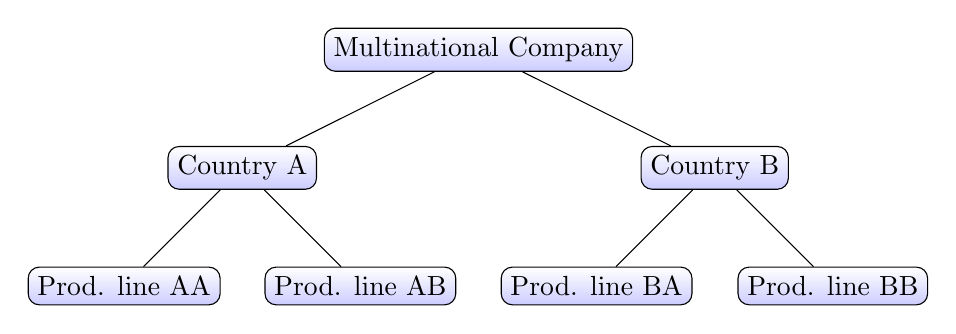
\begin{tikzpicture}[level/.style={sibling distance = 6cm/#1},
every node/.style = {shape=rectangle, rounded corners,
	draw, align=center,
	top color=white, bottom color=blue!20}]
\node {Multinational Company}
child {node {Country A} 
	child {node {Prod. line AA}}
	child {node {Prod. line AB}}
}
child {node {Country B} 
	child {node {Prod. line BA}}
	child {node {Prod. line BB}}
};
\end{tikzpicture}
\item[] 
\item \textbf{Hierarchical time series:} A collection of multiple time series that has an inherent aggregation structure 
\item Forecasts should add up. We call it \textit{coherent}
\item Why coherent forecasts?
% Coherent forecasts are important for budgetary allocations
\end{itemize}
\end{frame}
%-------------------%

%-----------------------------------------

%\section{Preliminaries}
\begin{frame}
\frametitle[]
%\frametitle{A first slide}

\begin{center}
	\Huge Preliminaries
\end{center}
\end{frame}
%----------------------------------------

\begin{frame}[noframenumbering]{Notations}
\begin{itemize}[<+-| alert@+>]
	\item[] 
	\begin{columns}
		\column{0.25\linewidth}
		\centering
		\begin{figure}
			\begin{center}
				\leaf{AA} \leaf{AB} 
				\branch{2}{A}
				\leaf{BA} \leaf{BB}
				\branch{2}{B}
				\branch{2}{Tot}
				\qobitree
			\end{center}
		\end{figure}
		
		\column{0.70\linewidth}
		\begin{itemize}[<+-| alert@+>]
			\item[]$\bm{y}_t = [y_{Tot,t},y_{A,t}, y_{B,t},y_{AA,t}, y_{AB,t}, y_{BA,t}, y_{BB,t}]^T$	
			\item[]$\bm{b}_t = [y_{AA,t}, y_{AB,t}, y_{BA,t}, y_{BB,t}]^T$	
			\item[]$m = 4$
			\item[]$n = 7$
			\item[]$\bm{S}=\begin{pmatrix} 1& 1 &1 &1  \\ 1 &1 & 0 &0\\   0&0 &1 & 1 \\  1 &0 & 0 &0\\  0 &1 & 0 &0\\0 &0 & 1 &0\\ 0 &0 & 0 &1\\  \end{pmatrix}$
		\end{itemize}	
	\end{columns} 
	\item Due to the aggregation nature of the hierarchy we have,
	$$\color{Maroon} \bm{y}_t = \bm{Sb}_t$$
	\item \textit{Coherent subspace:} $\mathfrak{s}=Span(\bm{S}), \quad \mathfrak{s} \subset \mathbb{R}^n$ 
	
\end{itemize}    
\end{frame}

%-------------------

\begin{frame}{Preliminaries: \textit{Coherent forecasts}}
\begin{itemize}
	\item[] 		
	%	\centering
	\begin{center}
		\vspace{-1.3cm}
		\includegraphics[scale=0.40]{Figures/3D_hierarchy}
	\end{center}
	\item Three dimensional hierarchy, $y_{Tot} = y_A + y_B$.
	\item $\vec{s}_1 = (1,1,0)'$ and $\vec{s}_2 = (1, 0, 1)'$ form a basis for $\mathfrak{s}$.
\end{itemize}    
\end{frame}

%-----------------------
%\begin{frame}{Preliminaries: \textit{Point forecasts reconciliation}}
%\begin{itemize}[<+-| alert@+>]
%\item Let $\hat{\bm{y}}_{t+h|t} \in \mathbb{R}^n$ be any set of incoherent point forecasts at time $t+h$.
%\begin{enumerate}
%	\item Pre-multiply $\hat{\bm y}_{t+h|t}$ by a $m\times n$ matrix $\bm G$ to obtain {\bf bottom} level series $\tilde{\bm b}_{t+h|t}={\bm G}\hat{\bm y}_{t+h|t}$ 
%	\item Pre-multiply $\tilde{\bm b}_{t+h|t}$ by a $n\times m$ matrix $\bm S$ to obtain ${\tilde{\bm y}}_{t+h|t}$, i.e. $\tilde{\bm y}_{t+h|t}={\bm S}\tilde{\bm b}_{t+h|t}$
%\end{enumerate}
%\item Choices of $\bm{G}$ defines reconciliation method
%\begin{itemize}
%	\item[$\bullet$] Bottom Up: ${\bm G}=\left(\bm{0}_{m\times n-m}~\bm{I}_{m\times m}\right)$ 
%	\item[]
%	\item[$\bullet$] MinT: ${\bm G}=\left(\bm{S}'\bm{W}_{T+h}^{-1}\bm{S}\right)^{-1}{\bm S'}\bm{W}_{T+h}^{-1}$\\
%	\citep{Wickramasuriya2018}
%	\begin{center}
%		\begin{block}{}
%			\begin{table}
%				\small
%				\centering %\setstretch{1.5}
%				\begin{tabular}{ll}
%					\toprule
%					\textbf{Method} & \textbf{Estimate of $\bm{W}_{T+h}$} \\
%					\midrule
%					OLS             &
%					$\bm{I}$  \\
%					MinT(Sample)    &
%					$\bm{\hat{W}}_{T+1}^{sam}$ \\
%					MinT(Shrink)    &
%					$\bm{\hat{W}}_{T+1}^{shr} = \tau\text{Diag}(\bm{\hat{W}}_{T+1}^{sam}) + (1-\tau)\bm{\hat{W}}_{T+1}^{sam}$ \\
%					MinT(WLS)       &
%					$\bm{\hat{W}}_{T+1}^{wls} = \text{Diag}(\bm{\hat{W}}_{T+1}^{shr})$  \\
%					\bottomrule
%				\end{tabular}
%			\end{table}
%		\end{block}
%	\end{center}
%
%	
%\end{itemize} 
%
%\end{itemize}    
%\end{frame}

\begin{frame}{Preliminaries: \textit{Point forecasts reconciliation}}
\begin{itemize}[<+-| alert@+>]
	\item Let $\hat{\bm y}\in\mathbb{R}^n$ be an incoherent forecast. Then, the reconciled forecasts $\tilde{\bm y}_{T+h}$ are given by,
	\begin{equation*}
	\color{Maroon}\tilde{\bm y}_{T+h} = \bm{SG}\hat{\bm y}_{T+h}
	\end{equation*}
	\item[]
	\begin{center}
		\begin{block}{}
			\begin{table}
				\small
				\centering %\setstretch{1.5}
				\begin{tabular}{lc}
					\toprule
					\textbf{Method} & \textbf{$\bm{G}$} \\
					\midrule
					BU             & $\left(\bm{0}_{m\times n-m}~\bm{I}_{m\times m}\right)$\\
					OLS             &
					$\left(\bm{S}'\bm{S}\right)^{-1}{\bm S'}$  \\
					WLS    &
					$\left(\bm{S}'\bm{\hat{W}}_{T+1}^{wls}\bm{S}\right)^{-1}\bm{S}'\bm{\hat{W}}_{T+1}^{wls}$ \\
					MinT(Shrink)    &
					$\left(\bm{S}'\bm{\hat{W}}_{T+1}^{shr}\bm{S}\right)^{-1}\bm{S}'\bm{\hat{W}}_{T+1}^{shr}$ \\
					\bottomrule
				\end{tabular}
			\end{table}
		\end{block}
		\begin{table}
			\small
			\centering %\setstretch{1.5}
			\begin{tabular}{lll}
				\toprule
				$\bm{\hat{W}}_{T+1}^{shr}$ & = & $\tau\text{Diag}(\bm{\hat{W}}_{T+1}^{sam}) + (1-\tau)\bm{\hat{W}}_{T+1}^{sam}$\\
				$\bm{\hat{W}}_{T+1}^{wls}$ & = & $\text{Diag}(\bm{\hat{W}}_{T+1}^{shr})$\\
				\bottomrule
			\end{tabular}
		\end{table}
	\end{center}
	
	
	
	
\end{itemize}
\end{frame}

%
%%-------------------

%
%-------------------------%

%%------------------------
%\section{Probabilistic forecasts in non-parametric framework: A bootstrap approach}
\begin{frame}
\frametitle[]
%\frametitle{A first slide}

\begin{center}
	\Huge Probabilistic forecasts for hierarchical time series
\end{center}
\end{frame}
%------------------------
\begin{frame}{Motivation}
\begin{itemize}[<+-| alert@+>]
	
	\item Lack of attention in probabilistic forecasts
	\begin{itemize}[<+-| alert@+>]
		\item[$\bullet$] \citet{BenTaieb2017}
		\item[$\bullet$] \citet{Jeon2018}
	\end{itemize}
	\item[]
	\item Probabilistic forecasts should reflect the inherent properties of real data. In particular, 
	\begin{itemize}[<+-| alert@+>]
		\item[$\star$] Aggregation structure
		\item[$\star$] Correlation structure
	\end{itemize}
	\item[]
	\item Extending the ``reconciliation" method into probabilistic framework
	
\end{itemize}
\end{frame}
%------------------%

\begin{frame}[noframenumbering]{Probabilistic forecast reconciliation}
\begin{itemize}[<+-| alert@+>]
	\item [$\bullet$] Often parametric densities are unavailable but we can simulate a sample from the predictive distribution.
	\item[]
	\item [$\bullet$] Suppose $\hat{\bm y}^{[1]}_{T+h},...,\hat{\bm y}^{[J]}_{T+h}$ is a sample from the incoherent predictive distribution.
	\item[]
	\item [$\bullet$] Then setting $\tilde{\bm y}^{[j]}_{T+h}=\bm{SG}\hat{\bm y}^{[j]}_{T+h}$ produces a sample from the reconciled predictive distribution with respect to $\bm{G}$.
\end{itemize}    
\end{frame}

%-----------------------


\begin{frame}{Non-parametric bootstrap approach}
\begin{enumerate}[<+-| alert@+>]
\item Fit univariate models at each node using data up to time $T$.
\item[]
\item Let $\bm{\Gamma}_{(T \times n)}=(\bm{e}_1,\bm{e}_2,\dots,\bm{e}_T)'$ be a matrix of in-sample residuals\\
where $\bm{e}_t=\bm{y}_t-\hat{\bm{y}}_t$. 
\item[]
\item Let $\bm{\Gamma}^b_{(H \times n)} = (\bm{e}^b_1,...,\bm{e}^b_H)'$ be a block bootstrap sample of size $H$ from $\bm{\Gamma}$.  
\item[]
\item Generate $h$-step ahead sample paths from the fitted models incorporating $\bm{\Gamma}^b$. Denote these by $\hat{\bm{y}}^b_{T+h}$, for $h=1,...,H$.
%\item[]
%\item  Repeat step 4 for $b = 1,...,B$ times.
%\item[]
%\item Setting $\tilde{\bm{y}}_{T+h,j}^b = \bm{SG}\hat{\bm{y}}_{T+h,j}^b$ produces a sample from the reconciled distribution.

\item[]
\item  Repeat step 3 and 4 for $b = 1,...,B$ times. Denote these as $\hat{\bm{\Upsilon}}_{T+h}=(\hat{\bm{y}}^1_{T+h},...,\hat{\bm{y}}^B_{T+h})'$ for all $h$.
\item[]
\item Setting $\tilde{\bm{\Upsilon}}_{T+h} = \bm{SG}\hat{\bm{\Upsilon}}'_{T+h}$ produces a sample from the reconciled distribution.

\seti
\end{enumerate}
\end{frame}
%
%
%\subsection{Monte-Carlo simulation in non-parametric framework}

\begin{frame}{Optimal reconciliation of future paths}
\begin{itemize}[<+-| alert@+>]
\item We propose to find an optimal $\bm{G}_h$ matrix by minimizing Energy score. 
\begin{equation*}
\operatornamewithlimits{argmin}_{\bm{G}_h} \quad \E_{\bm{Q}}[eS(\tilde{\bm{F}}, \bm{y}_{T+h})], \quad  \tilde{\bm{F}} := \tilde{\bm{\Upsilon}}_{T+h} = \bm{SG}_h\hat{\bm{\Upsilon}}'_{T+h}
\end{equation*}
where, \begin{align*}
\text{eS}(\tilde{\bm{F}},\bm{y}_{T+h}) = 
\E_{\tilde{\bm{F}}}
\|\tilde{\bm{Y}}_{T+h}-\bm{y}_{T+h}\|^\alpha -
\frac{1}{2}\E_{\tilde{\bm{F}}}\|\tilde{\bm{Y}}_{T+h}-\tilde{\bm{Y}}^*_{T+h}\|^\alpha,\\ \alpha \in (0,2]
\end{align*}

\end{itemize}
\end{frame}

%---------------------
\begin{frame}{Optimal reconciliation of future paths}
\begin{itemize}[<+-| alert@+>]
	
	\item Monte-Carlo approximation to the objective function is, 
	\begin{block}{}
		\begin{align*}
		\operatornamewithlimits{argmin}_{\bm{G}_h} \quad \sum_{i=1}^{N}\Big\{\frac{1}{B}\sum_{b=1}^{B}||\bm{SG}_h&\hat{\bm{y}}_{T+h,i}^b -\bm{y}_{T+h}||-\\
		&\frac{1}{2(B-1)}\sum_{b=1}^{B-1}||\bm{SG}_h(\hat{\bm{y}}_{T+h,i}^b -\hat{\bm{y}}_{T+h,i,}^{b+1})||\Big\}
		\end{align*}
	\end{block}
\end{itemize}
\end{frame}

%%-------------------------------
\begin{frame}{Optimal reconciliation of future paths \textit{Cont.}}
\begin{itemize}[<+-| alert@+>]
\item We impose the following structure to the $\bm{G}_h$ matrix
\begin{equation}\label{eq:2}
\bm{G}_h=\left(\bm{S}'\bm{W}_h\bm{S}\right)^{-1}{\bm S'}\bm{W}_h
\end{equation}
\item We propose four methods to optimise $\bm{G}_h$
\begin{enumerate}
\item[]
\item[] \textbf{\color{Maroon}Method 1:} Optimising $\bm{W}_h$
\item[] 
\item[] \textbf{\color{Maroon}Method 2:} Optimising Cholesky decomposition of $\bm{W}_h$
\item[] \textbf{\color{White}Method 2:} $\bm{W}_h=\bm{R_h'R_h}$ where $\bm{R}_h$ is an upper triangular matrix 
\item[]
\item[] \textbf{\color{Maroon}Method 3:} Optimising Cholesky of $\bm{W}_h$ - restricted for scaling
\item[] \textbf{\color{White}Method 3:}$\bm{W}_h=\bm{R'_hR_h} \quad \text{s.t} \quad \bm{i'W_hi}=1$ where $\bm{i}=(1,0,..,0)'$
\item[] 
\item[] \textbf{\color{Maroon}Method 4:} Optimising $\bm{G}_h$ such that $\bm{G}_h\bm{S=I}$

\end{enumerate}
\end{itemize}
\end{frame}

%------------------------

\begin{frame}{Monte-Carlo Simulation}
\begin{itemize}
\item Data generating process
\item[] 
\begin{columns}
\column{0.4\linewidth}
\centering
\begin{figure}
\begin{center}
\leaf{A} \leaf{B} 
\branch{2}{Tot}
\qobitree
\end{center}
\end{figure}

\column{0.4\linewidth}
\begin{figure}
\begin{center}
\leaf{AA} \leaf{AB} 
\branch{2}{A}
\leaf{BA} \leaf{BB}
\branch{2}{B}
\branch{2}{Tot}
\qobitree
\end{center}
\end{figure}
\end{columns} 
\item[]
\item DGP was designed such that we have much noisier series in the bottom level.

\end{itemize}
\end{frame}

%------------------

\begin{frame}{Monte-Carlo Simulation}

\includegraphics[scale=0.4]{Figures/Optimisation_TestingG.pdf}

\end{frame}

%------------------%

%\begin{frame}{Monte-Carlo Simulation \textit{Cont.}}
%\begin{itemize}
%\item Simulation setup: 
%\begin{itemize}[<+-| alert@+>]
%\item [$\bullet$] First 2500 observations were generated.
%\item [$\bullet$] Fit Univariate ARIMA models for a rolling window of 500 observations.
%\item [$\bullet$] $B=1000$ of $h=1,2,3$ steps-ahead bootstrap future paths generated.
%\item [$\bullet$] Training window is rolled one observation ahead and process was repeated until $N=100$ incoherent, $h=1,2,3$ steps-ahead future paths were generated.
%\item [$\bullet$] We find the optimal $\bm{G}_h$ for $h=1,2,3$ that reconciles $h$-step-ahead future paths giving minimal average Energy score. 
%\item [$\bullet$] This optimal $\bm{G}_h$ is then used to reconcile the incoherent future paths for the test set.
%\item [$\bullet$] The Process was repeated 1000 times and average scores were calculated for the test set.
%\end{itemize}
%\end{itemize}
%\end{frame}
%------------------%

\begin{frame}{Monte-Carlo Simulation \textit{Cont.}}
\begin{itemize}
\item []
\begin{table}

\resizebox{\linewidth}{!}{
\small
\begin{tabular}{@{}lSSSSSSSS@{}}
\toprule
\multicolumn{1}{c}{Optimisation} &
\multicolumn{4}{c}{\text{Hierarchy 1}} & 
\multicolumn{4}{c}{\text{Hierarchy 2}} \\
\cmidrule(lr){2-5} \cmidrule(lr){6-9} 
\multicolumn{1}{c}{method} & \multicolumn{2}{c}{$h=1$} & \multicolumn{2}{c}{$h=3$} & \multicolumn{2}{c}{$h=1$} & \multicolumn{2}{c}{$h=3$} \\
\cmidrule(lr){2-3} \cmidrule(lr){4-5} \cmidrule(lr){6-7} \cmidrule(lr){8-9} 
& \text{ES} & \text{VS} & \text{ES} & \text{VS} & \text{ES} & \text{VS} & \text{ES} & \text{VS} \\   

\midrule
Method 1    			& 2.48 & 0.11 & 2.75 & 0.11 & 5.36 & 1.21 & 5.83 & 1.38  \\
Method 2    			& 2.48 & 0.11 & 2.75 & 0.11 & 5.37 & 1.21 & 5.83 & 1.37  \\
Method 3 				& 2.48 & 0.11 & 2.75 & 0.11 & 5.37 & 1.21 & 5.83 & 1.37  \\
Method 4    			& 2.48 & 0.11 & 2.75 & 0.11 & 5.38 & 1.21 & 5.83 & 1.38  \\
\bottomrule

\end{tabular}
}
\end{table}
\item[]
\item Parameterisation does not matter
\end{itemize}
\end{frame}

%------------------%

\begin{frame}{Monte-Carlo Simulation \textit{Cont.}}
\begin{itemize}[<+-| alert@+>]
\item Comparison with point forecast reconciliation methods.
\item[]
\begin{table}
\resizebox{\linewidth}{!}{
\small
%\begin{tabular}{@{}lSSSSSSSS@{}}
\begin{tabular}{@{}lllllllll@{}}
\toprule
\multicolumn{1}{c}{Reconciliation} &
\multicolumn{4}{c}{\text{Hierarchy 1}} & 
\multicolumn{4}{c}{\text{Hierarchy 2}} \\
\cmidrule(lr){2-5} \cmidrule(lr){6-9} 
\multicolumn{1}{c}{method} & \multicolumn{2}{c}{$h=1$} & \multicolumn{2}{c}{$h=3$} & \multicolumn{2}{c}{$h=1$} & \multicolumn{2}{c}{$h=3$} \\
\cmidrule(lr){2-3} \cmidrule(lr){4-5} \cmidrule(lr){6-7} \cmidrule(lr){8-9} 
& \text{ES} & \text{VS} & \text{ES} & \text{VS} & \text{ES} & \text{VS} & \text{ES} & \text{VS} \\   

\midrule
Optimal $\bm{G}$   	& 2.48* & 0.106 & 2.75* & 0.106 & 5.36* & 1.21* & 5.83* & 1.38*\\
MinT(Shrink)    	& 2.47* & 0.105 & 2.74* & 0.105 & 5.33* & 1.19* & 5.77* & 1.34*\\			
WLS   				& 2.46* & 0.105 & 2.74* & 0.105 & 5.43* & 1.23 & 5.98* & 1.40* \\
OLS 				& 2.54* & 0.105 & 2.80* & 0.105 & 5.51* & 1.23 & 5.98* & 1.40*\\
\textit{Base} 		& $\textit{2.67}$ & $\textit{0.105}$ & $\textit{2.94}$ & $\textit{0.105}$ & $\textit{5.71}$ & $\textit{1.28}$ & $\textit{6.27}$ & $\textit{1.49}$\\   			
\bottomrule
\multicolumn{9}{l}{\text{``*'' indicates if the average score for a particular reconciliation method is significantly }}\\
\multicolumn{9}{l}{\text{different from that of base forecasts.}}

\end{tabular}
}
\end{table}
\item[]
\item Reconciliation methods perform better than Base forecasts.
\item[]
\item MinT(Shrink) is at least as good as Optimal method. Thus going forward with MinT projection. 

\end{itemize}
\end{frame}

%---------------------



%\section{Forecasting Australian domestic tourism flows}
\begin{frame}
\frametitle[]
%\frametitle{A first slide}

\begin{center}
	\Huge Forecasting Australian domestic tourism flows
\end{center}
\end{frame}
%------------------%

\begin{frame}[noframenumbering]{Forecasting Australian domestic tourism flows}
\begin{itemize}[<+-| alert@+>]
\item[] 
\begin{block}{Geographical hierarchical structure for Australia}
\begin{table}
\small
\centering %\setstretch{1.5}
\begin{tabular}{lc}
\toprule
\textbf{Level} & \textbf{No.Series per level} \\
\midrule
\text{Total (Australia)}  	&	{$1$}  \\
\text{Level-1 (States)}    	&	{$7$}  \\
\text{Level-2 (Zones)}    	&	{$27$} \\
\text{Level-3 (Regions)}    &	{$75$} \\
\bottomrule
\end{tabular}
\end{table}
\end{block}
\item Data: monthly ``overnight trips" over the period January 1998 - December 2017
\item Source of data: National Visitor Survey (NVS) [Tourism Research Australia]
\end{itemize}
\end{frame}


%------------------%

\begin{frame}{Forecasting Australian domestic tourism flows}
\begin{itemize}[<+-| alert@+>]
	\item \textbf{Analysis set up:}
\begin{itemize}[<+-| alert@+>]
	\item[$\bullet$] First training sample is set from 1998:Jan to 2006:Apr 
	\item[$\bullet$] Univariate ARIMA models were fitted for each series in the hierarchy.
	\item[$\bullet$] Reconciled probabilistic forecasts were produced for six months ahead (2006:May to 2006:Oct)
	\item[$\bullet$] Then the training window is rolled by one month ahead at a time.
	\item[$\bullet$] This leads to 140 1-step-ahead, 139 2-steps-ahead, through 135 6-step-ahead forecasts available for evaluation. 
\end{itemize}
\end{itemize}
\end{frame}

%-------------------


%-----------------%

\begin{frame}{Results}

	\textit{Overall probabilistic forecast performance}
	\space
	\centering
	\includegraphics[scale=0.5]{Figures/Results/Overall-MultivS}
	

\end{frame}

%---------------


\begin{frame}{Results}

\textit{Probabilistic forecast performance for different levels}
\centering
\includegraphics[scale=0.53]{Figures/Results/Stat-Zon-Reg-MultivS}


\end{frame}


%\section{Conclusions}
\begin{frame}
\frametitle[]
%\frametitle{A first slide}

\begin{center}
	\Huge Conclusions\\
	\end{center}
\end{frame}

\begin{frame}[noframenumbering]{Conclusions}
\begin{itemize}[<+-| alert@+>]
%\item Linear reconciliation involves two steps
%\item[] Step 1: Transform coordinates of incoherent prob. forecasts 
%\item[] Step 2: Marginalize over the null space of the coherent subspace
%\item[]
\item We introduce a novel non-parametric bootstrap approach for producing reconciled probabilistic forecasts
\item[]
\item Simulation study evident that the optimal reconciliation with respect to energy score is equivalent to reconciling each sample path via MinT approach
\item[]
\item We apply this non-parametric bootstrap approach to obtain coherent probabilistic forecasts for domestic tourism flow in Australia  




\end{itemize}
\end{frame}

%
%
%
%%%%%%START%%%%%
%%--------------------------------------------
%
%
%%--------------------------------
%
%
\begin{frame}[allowframebreaks]{References}
\printbibliography
\end{frame}
%
\begin{frame}{}
\begin{center}
	
	\begin{LARGE} \bf THANK YOU!\end{LARGE} \\[1cm]
	{\color{monashblue} \bf Email}: \texttt{puwasala.gamakumara@monash.edu}
\end{center}
\end{frame}

\begin{frame}[noframenumbering]
\frametitle[]
%\frametitle{A first slide}

\begin{center}

\Huge Appendix
	
\end{center}
\end{frame}

\begin{frame}[noframenumbering]{Appendix: \textit{Probabilistic forecasts evaluation}}\hypertarget{ScoringRules}{\hyperlink{backtoScoringRule}{\beamerbutton{A2}}}
%{\beamerreturnbutton{A1}}
\begin{itemize}
	\item[]
	\begin{block}{}
		\begin{table}
			\small
			\centering %\setstretch{1.5}
			\resizebox{\linewidth}{!}{
				\begin{tabular}{lll}
					\textbf{Energy score}  & & \citep{Gneiting2008}\\
					$\text{eS}(\breve{\bm{Y}}_{T+h},\bm{y}_{T+h})$&=&
					$
					\E_{\breve{\bm{F}}}
					\|\breve{\bm{Y}}_{T+h}-\bm{y}_{T+h}\|^\alpha -
					\frac{1}{2}\E_{\breve{\bm{F}}}\|\breve{\bm{Y}}_{T+h}-\breve{\bm{Y}}^*_{T+h}\|^\alpha, \quad \alpha \in (0,2]$ \\
					&&\\
					%&& $\alpha \in (0,2]$\\ 
					\textbf{Log score}& & \citep{Gneiting2007}\\
					
					$\text{LS}(\breve{\bm{F}},\bm{y}_{T+h})$ & = & $-\log {\breve{\bm{f}}(\bm{y}_{T+h})}$\\
					&&\\
					\textbf{Variogram score} & & \citep{SCHEUERER2015}\\
					
					$\text{VS}(\breve{\bm{F}}, \bm{y}_{T+h})$ &=&
					$\sum\limits_{i=1}^{n}
					\sum\limits_{j=1}^{n}
					w_{ij}\Big(|y_{T+h,i} - y_{T+h,j}|^p-\E_{\breve{\bm{F}}}|\breve{Y}_{T+h,i}-\breve{Y}_{T+h,j}|^p\Big)^2$\\ 
					
					&&\\
					\textbf{CRPS} & & \citep{Gneiting2007}\\
					
					$\text{CRPS}(\breve{F}_i,y_{T+h,i})$ &=&
					$\E_{\breve{F}_i}|\breve{Y}_{T+h,i}-y_{T+h,i}| - \frac{1}{2}\E_{\breve{F}_i}|\breve{Y}_{T+h,i}-\breve{Y}^*_{T+h,i}|$\\ 
					
					
				\end{tabular}
			}
		\end{table}
		
	\end{block}
	\begin{table}
		\small
		\centering %\setstretch{1.5}
		\begin{tabular}{lll}
			\toprule
			$\breve{\bm{Y}}_{T+h}$ and $\breve{\bm{Y}}^*_{T+h}$ & : & Independent random vectors from the coherent \\
			& & forecast distribution $\breve{\bm{F}}$.\\
			$\bm{y}_{T+h}$ & : &Vector of realizations. \\
			$\breve{Y}_{T+h,i}$ and $\breve{Y}_{T+h,j}$ & : & $i$th and $j$th components of the vector $\breve{\bm{Y}}_{T+h}$ \\
			$w_{ij}$ & : & Non-negative weights\\
			\bottomrule
		\end{tabular}
	\end{table}
	
\end{itemize}

\end{frame}

%\begin{frame}[noframenumbering]{Appendix}
%\begin{itemize}
%	\item \hypertarget{OLS}{\beamerreturnbutton{A1}} Shrinkage estimatorfor 1-step ahead base forecast errors
%	$$
%	\hat{\bm{\Sigma}}_{T+1}^{shr} = \tau\hat{\bm{\Sigma}}_{T+1}^D + (1-\tau)\hat{\bm{\Sigma}}_{T+1},
%	$$
%	where $\hat{\bm{\Sigma}}_{T+1}^D$ is the diagonal matrix comprising diagonal entries of $\hat{\bm{\Sigma}}_{T+1}$ and $$\tau = \frac{\sum_{i \ne j}\hat{Var}(\hat{r}_{ij})}{\sum_{i \ne j}\hat{r}_{ij}^2}$$ is a shrinkage parameter. $\hat{r}_{ij}$ is the $ij$-th element of sample correlation matrix.  In this estimation, the off-diagonal elements of 1-step ahead sample covariance matrix will be shrunk to zero depending on the sparsity.
%	
%\end{itemize}
%\end{frame}


%\begin{frame}[noframenumbering]{Monte-Carlo simulation - Gaussian}
%\begin{itemize}[<+-| alert@+>]
%\item \textbf{Data generating process}\hypertarget{Simulation_Gaussian}{\beamerreturnbutton{A1}}
%
%\begin{figure}
%\begin{center}
%\leaf{AA} \leaf{AB} 
%\branch{2}{A}
%\leaf{BA} \leaf{BB}
%\branch{2}{B}
%\branch{2}{Tot}
%\qobitree
%\end{center}
%\end{figure}
%\item DGP was designed such that we have noisier series in the bottom levels than in the aggregate levels  
%
%\item \textbf{Simulation setup}
%\begin{itemize}[<+-| alert@+>]
%\item[$\bullet$] 501 observations were generated
%\item[$\bullet$] Univariate ARIMA models were fitted to the first 500 observations and 1- step ahead incoherent forecasts were generated
%\item[$\bullet$] Mean and variance forecasts of incoherent Gaussian densities were reconciled through different estimates of $\bm{R}'_\bot$
%\item[$\bullet$] This process was replicated using 1000 different series from the same (DGP)
%\end{itemize}
%
%\end{itemize} 
%\end{frame}
%

%----------------%
%\begin{frame}[noframenumbering]{Monte-Carlo simulation \textit{Cont..}}
%\begin{itemize}[<+-| alert@+>]
%\item Comparison of reconciled vs bottom-up Gaussian forecasts
%\begin{table}
%\resizebox{\linewidth}{!}{
%\begin{tabular}{@{}lSSSSSS@{}}
%\toprule
%Forecasting &
%\multicolumn{2}{c}{\text{Energy score}} &
%\multicolumn{2}{c}{\text{Log score}} &
%\multicolumn{2}{c}{\text{Variogram score}} \\
%\cmidrule(lr){2-3} \cmidrule(lr){4-5} \cmidrule(l){6-7}
%method &
%\text{Average score} & \text{Skill score (\%)} &
%\text{Average score} & \text{Skill score (\%)} &
%\text{Average score} & \text{Skill score (\%)}\\
%\midrule
%MinT(Shrink) &  {\cellcolor{green!25}} 7.47 &  {\cellcolor{green!25}} 10.11 &  {\cellcolor{green!25}} 11.34 &     {\cellcolor{green!25}} 6.44 & {\cellcolor{green!25}} 3.05 &  {\cellcolor{green!25}} 4.69 \\
%MinT(Sample) &  {\cellcolor{green!25}} 7.47 &  {\cellcolor{green!25}} 10.11 &  {\cellcolor{green!25}} 11.33 &    {\cellcolor{green!25}} 6.52 & {\cellcolor{green!25}} 3.05 &   {\cellcolor{green!25}} 4.69 \\
%MinT(WLS)    &  7.91 &   4.81 &  12.64 &    -4.29 & 3.23 &  -0.94 \\
%OLS          & 10.14 & -22.02 & 135.13 & -1014.93 & 4.60 & -43.75 \\
%Bottom up    &  8.31 &        &  12.12 &          & 3.20 &        \\
%\bottomrule
%\text{Note:}&\multicolumn{6}{l}{\textit{Positive(/negative) entry in ``Skill score (\%)" column represent the percentage increase(/decrease) of }}\\
%&\multicolumn{6}{l}{\textit{preferred forecasting method over Bottom-up method.}}\\
%
%\bottomrule
%\end{tabular}
%}
%\end{table}
%
%\end{itemize} 
%\end{frame}

%-----------------%
%\begin{frame}[noframenumbering]{Monte-Carlo simulation \textit{Cont..}}
%\begin{itemize}
%\item Comparison of coherent vs incoherent Gaussian forecasts
%\begin{table}
%\centering\small
%\resizebox{\linewidth}{!}{
%\begin{tabular}{@{}lSSSSSS@{}}
%\toprule
%Forecasting &
%\multicolumn{2}{c}{\text{Total}} &
%\multicolumn{2}{c}{\text{Series - A}} &
%\multicolumn{2}{c}{\text{Series - B}} \\
%\cmidrule(lr){2-3} \cmidrule(lr){4-5} \cmidrule(l){6-7}
%method      &  CRPS   & LogS    & CRPS   & LogS     & CRPS   & LogS     \\
%\midrule
%MinT(Shrink) & {\cellcolor{green!25}} 1.12   & {\cellcolor{green!25}} 0.34    & {\cellcolor{green!25}} 10.07  & {\cellcolor{green!25}} 2.93     & {\cellcolor{green!25}} 5.41   & {\cellcolor{green!25}} 1.52     \\
%MinT(Sample) & {\cellcolor{green!25}} 1.12   & {\cellcolor{green!25}} 0.34    & {\cellcolor{green!25}} 10.07  & {\cellcolor{green!25}} 2.93     & {\cellcolor{green!25}} 5.41   & {\cellcolor{green!25}} 1.52     \\
%MinT(WLS)    & -2.61  & -2.02   & 5.28   & -4.40    & 2.70   & -4.24    \\
%OLS          & -38.06 & -698.99 & -24.70 & -1368.33 & -24.86 & -1159.09 \\
%Bottom up    & -89.55 & -21.83  & -8.87  & -2.35    & -9.46  & -2.73    \\
%\midrule
%\textit{Incoherent} & $\textit{2.68}$ & $\textit{2.97}$ & $\textit{4.17}$ & $\textit{3.41}$ & $\textit{3.70}$ & $\textit{3.30}$ \\
%\bottomrule
%
%\end{tabular}
%}
%\end{table}
%
%\begin{table}
%\resizebox{\linewidth}{!}{
%\centering\small
%\begin{tabular}{@{}lSSSSSSSS@{}}
%\toprule
%Forecasting &
%\multicolumn{2}{c}{\text{Series - AA}} &
%\multicolumn{2}{c}{\text{Series - AB}} &
%\multicolumn{2}{c}{\text{Series - BA}} &
%\multicolumn{2}{c}{\text{Series - BB}} \\
%\cmidrule(lr){2-3} \cmidrule(lr){4-5} \cmidrule(lr){6-7} \cmidrule(l){8-9}
%method       & CRPS   & LogS    & CRPS   & LogS    & CRPS   & LogS    & CRPS   & LogS \\
%\midrule
%MinT(Shrink) & {\cellcolor{green!25}} 8.71   & {\cellcolor{green!25}} 2.71    & {\cellcolor{green!25}} 10.57  & {\cellcolor{green!25}} 3.04    & {\cellcolor{green!25}} 5.95   & {\cellcolor{green!25}} 1.86    & {\cellcolor{green!25}} 7.91   & {\cellcolor{green!25}} 2.46 \\
%MinT(Sample) & {\cellcolor{green!25}}8.71   & {\cellcolor{green!25}} 2.71    & {\cellcolor{green!25}} 10.57  & {\cellcolor{green!25}} 3.04    & {\cellcolor{green!25}} 5.95   & {\cellcolor{green!25}} 1.86    & {\cellcolor{green!25}} 8.19   & {\cellcolor{green!25}} 2.46 \\
%MinT(WLS)    & 5.54   & 0.30    & 5.96   & 0.30    & 2.43   & -0.62   & 5.08   & 0.62 \\
%OLS          & -22.43 & -931.63 & -22.49 & -886.32 & -26.01 & -834.67 & -23.45 & -812.92 \\
%\midrule
%\textit{Incoherent} & $\textit{3.79}$ & $\textit{3.32}$ & $\textit{3.69}$ & $\textit{3.29}$ & $\textit{3.46}$ & $\textit{3.23}$ & $\textit{3.54}$ & $\textit{3.25}$ \\
%\bottomrule
%\text{Note:}&\multicolumn{8}{l}{\textit{``Incoherent" row represents the average score for incoherent forecasts.}}\\
%&\multicolumn{8}{l}{\textit{Each entry above this row represent the percentage skill score with reference to the Incoherent forecasts.}}\\
%
%\bottomrule
%\end{tabular}
%}
%\end{table}
%
%\end{itemize} 
%\end{frame}

%--------------------

%\begin{frame}[noframenumbering]{Monte-Carlo simulation - bootstrap approach} \hypertarget{Simulation_NonPara}{\beamerreturnbutton{A2}}
%\begin{itemize}[<+-| alert@+>]
%\item \textbf{Data generating process}
%\begin{figure}
%\begin{center}
%\leaf{AA} \leaf{AB} 
%\branch{2}{A}
%\leaf{BA} \leaf{BB}
%\branch{2}{B}
%\branch{2}{Tot}
%\qobitree
%\end{center}
%\end{figure}
%\item DGP was designed such that we have noisier series in the bottom levels than in the aggregate levels  
%
%
%\item \textbf{Simulation setup}
%\begin{itemize}[<+-| alert@+>]
%\item[$\bullet$] $1510$ observations were generated
%\item[$\bullet$] Univariate ARIMA models were fitted using a rolling window of $500$ observations as the training set
%\item[$\bullet$] $5000$ reconciled future sample paths were generated for forecast horizons $h=1,...,5$ 
%\item[$\bullet$] The training window was rolled one observation ahead and the process repeated until we get 1000 reconciled future sample paths
%%\includegraphics[scale=0.40]{Rolling_window}	
%\end{itemize}
%
%
%\end{itemize}
%\end{frame}

%------------------------------%

%\begin{frame}[noframenumbering]{Monte-Carlo simulation - bootstrap approach}
%\begin{itemize}[<+-| alert@+>]
%
%\item Comparison of reconciled vs bottom-up forecasts
%\includegraphics[scale=0.60]{Figs/Bootstrap_MVScore}
%\end{itemize}
%\end{frame}
%%------------------
%\begin{frame}[noframenumbering]{Analyzing the predictive performance of probabilistic forecasts in a non-parametric framework}
%\begin{itemize}[<+-| alert@+>]
%
%\item Comparison of coherent vs incoherent forecasts\\
%\includegraphics[scale=0.60]{Figs/Bootstrap_UnivariateAna}
%\end{itemize}
%\end{frame}

%-----------------%



%\begin{frame}[noframenumbering]{Appendix}
%
%\begin{itemize}
%\item \hypertarget{OLS}{\beamerreturnbutton{A1}} \textbf{Optimal reconciliation approach}
%\begin{itemize}
%\item[$\bullet$] based on a regression, \\
%$\hat{\bm{y}}_{T+h} = \bm{S\beta}_{T+h} + \bm{\varepsilon}_{T+h}$
%\end{itemize}
%	\begin{block}{}
%$ \color{Maroon} OLS: \quad \bm{P} = (\bm{S}^T\bm{S})^{-1}\bm{S}^T$
%\end{block}
%\end{itemize}
%\end{frame}
%
%

%\begin{frame}[noframenumbering]{Appendix}
%\begin{itemize}[<+-| alert@+>]
%	\item[] \hypertarget{Prob_Gauss}{\beamerreturnbutton{A1}}
%	\item By substituting the Gaussian distribution function for $\hat{\bm{f}}(\cdot)$ in $\bm{f_B}(\cdot)$ we get, 
%	\begin{align*}
%	\bm{f_B}(\cdot)
%	& =
%	\frac{1}{(2\pi)^{\frac{n}{2}}\Big|\PQ\bm{{W}_{t+h}}\PQ'\Big|^{\frac{1}{2}}}
%	\exp \Big\{-\frac{1}{2} \begin{pmatrix}\tilde{\bm{b}}_{t+h} - \bm{P}\bm{\hat{y}}_{t+h}\\ \bm{t}_{t+h}- \bm{Q}\bm{\hat{y}}_{t+h}\end{pmatrix}' \\
%	& \Big[\PQ\bm{{W}_{t+h}}\PQ'\Big]^{-1}\begin{pmatrix}\tilde{\bm{b}}_{t+h} - \bm{P}\bm{\hat{y}}_{t+h}\\ \bm{t}_{t+h}- \bm{Q}\bm{\hat{y}}_{t+h}\end{pmatrix} \Big\}.
%	\end{align*}
%	where$$
%	(\bm{S} ~ \vdots~ \bm{R})^{-1} =
%	\begin{pmatrix}(\bm{R}'_\bot \bm{S})^{-1}\bm{R}'_\bot \\ \cdots \\ (\bm{S}'_\bot \bm{R})^{-1}\bm{S}'_\bot \end{pmatrix} =
%	\begin{pmatrix}
%	\bm{P} \\\bm{Q}
%	\end{pmatrix},
%	$$
%	and $\bm{P}=(\bm{R}'_\bot \bm{S})^{-1}\bm{R}'_\bot$ and $\bm{Q}=(\bm{S}'_\bot \bm{R})^{-1}\bm{S}'_\bot$.
%	
%\end{itemize}    
%
%\end{frame}
%
%%------------------------%
%\begin{frame}[noframenumbering]{Appendix}
%\begin{itemize}
%	\item \hypertarget{Shrinkage}{\beamerreturnbutton{A2}} Shrinkage estimator for 1-step ahead base forecast errors
%	$$
%	\hat{\bm{\Sigma}}_{T+1}^{shr} = \tau\hat{\bm{\Sigma}}_{T+1}^D + (1-\tau)\hat{\bm{\Sigma}}_{T+1},
%	$$
%	where $\hat{\bm{\Sigma}}_{T+1}^D$ is the diagonal matrix comprising diagonal entries of $\hat{\bm{\Sigma}}_{T+1}$ and $$\tau = \frac{\sum_{i \ne j}\hat{Var}(\hat{r}_{ij})}{\sum_{i \ne j}\hat{r}_{ij}^2}$$ is a shrinkage parameter. $\hat{r}_{ij}$ is the $ij$-th element of sample correlation matrix.  In this estimation, the off-diagonal elements of 1-step ahead sample covariance matrix will be shrunk to zero depending on the sparsity.
%	
%\end{itemize}
%\end{frame}
%
%%-----------------%
%
%\begin{frame}[noframenumbering]{Monte-Carlo simulation}
%\begin{itemize}[<+-| alert@+>]
%	\item \textbf{Data generating process}\hypertarget{Simulation}{\beamerreturnbutton{A3}}
%	\begin{columns}
%		\column{0.25\linewidth}
%		\centering
%		\begin{figure}
%			\begin{center}
%				\leaf{AA} \leaf{AB} 
%				\branch{2}{A}
%				\leaf{BA} \leaf{BB}
%				\branch{2}{B}
%				\branch{2}{Tot}
%				\qobitree
%			\end{center}
%		\end{figure}
%		
%		\column{0.70\linewidth}
%		\begin{itemize}[<+-| alert@+>]
%			\item $\{w_{AA,t},w_{AB,t},w_{BA,t},w_{BB,t}\} \sim ARIMA(p,d,q)$ 	
%			\item	$p \in \{1,2\}$ and $d \in \{0,1\}$
%			\item $\{\epsilon_{AA,t},\epsilon_{AB,t},\epsilon_{BA,t},\epsilon_{BB,t}\} \sim \mathcal{N}(\bm{0}, \bm{\Sigma})$
%			\item Parameters for $AR$ and $MA$ components were randomly and uniformly generated from $[0.3,0.5]$ and $[0.3,0.7]$ respectively
%			
%		\end{itemize}	
%	\end{columns} 
%	
%	\item[]
%	\item $\bm{y}_t$ are then generated as follows
%	\item[]\begin{table}
%		\small
%		\centering %\setstretch{1.5}
%		\resizebox{\linewidth}{!}{
%			\begin{tabular}{lll}
%				\toprule
%				\textbf{Bottom level} & \textbf{Aggregate level 1} & \textbf{Total}      \\
%				\midrule
%				$y_{AA,t} = w_{AA,t} + u_t - 0.5v_t$ & $y_{A,t} = w_{AA,t} + w_{AB,t} - v_t$ & $y_{Tot,t} = w_{AA,t} + w_{AB,t} + w_{BA,t} + w_{BB,t}$\\
%				$y_{AB,t} = w_{AB,t} - u_t - 0.5v_t$ & $y_{B,t} = w_{BA,t} + w_{BB,t} + v_t$ &\\
%				$y_{BA,t} = w_{BA,t} + u_t + 0.5v_t$ & &\\
%				$y_{BB,t} = w_{BB,t} - u_t + 0.5v_t$ & &\\
%				\bottomrule
%			\end{tabular}
%		}
%	\end{table}
%	
%	
%\end{itemize} 
%\end{frame}
%%
%
%\begin{frame}[noframenumbering]{Monte-Carlo simulation \textit{Cont..}}
%\begin{itemize}[<+-| alert@+>]
%\item To get less noisier series at aggregate levels, we choose $\bm{\Sigma}, \sigma^2_u$ and $\sigma^2_v$ such that,
%\begin{table}
%	\small
%	\centering %\setstretch{1.5}
%	\resizebox{\linewidth}{!}{
%		\begin{tabular}{l}
%			$
%			\text{Var}(\epsilon_{AA,t}+\epsilon_{AB,t}+\epsilon_{BA,t}+\epsilon_{BB,t}) \le \text{Var}(\epsilon_{AA,t}+\epsilon_{AB,t}-v_t) \le \text{Var}(\epsilon_{AA,t}+u_t-0.5v_t),
%			$\\
%		\end{tabular}
%	}
%\end{table}
%
%\item Thus we choose,
%$\bm{\Sigma} =
%\begin{pmatrix}
%5.0 & 3.1 & 0.6 & 0.4 \\
%3.1 & 4.0 & 0.9 & 1.4 \\
%0.6 & 0.9 & 2.0 & 1.8 \\
%0.4 & 1.4 & 1.8 & 3.0 \\
%\end{pmatrix}$,
%$\sigma^2_u = 19$ and $\sigma^2_u = 18$.
%
%
%\end{itemize} 
%\end{frame}
%%
%
%\begin{frame}[noframenumbering]{Sample version of the scoring rules}
%\begin{itemize}[<+-| alert@+>]
%	
%	\item For a possible finite sample of size $B$ from the multivariate forecast density $\breve{\bm{F}}$, the variogram score is defined as,
%	\begin{table}
%	\small
%	$\text{VS}(\breve{\bm{F}}, \bm{y}_{T+h}) = \displaystyle\sum_{i=1}^{n}\displaystyle\sum_{j=1}^{n}w_{ij}\left(|y_{T+h,i} - y_{T+h,j}|^p - \frac{1}{B} \displaystyle\sum_{k=1}^{B} |\breve{Y}^k_{T+h,i}-\breve{Y}^k_{T+h,j}|^p\right)^2$
%	\end{table}
%		
%	
%\end{itemize} 
%\end{frame}
%%

%-------------------%




\end{document}
